\documentclass[14pt, a4paper]{article}

\usepackage[utf8]{inputenc}
\usepackage[T2A]{fontenc}

\usepackage{graphicx}
\graphicspath{ {images/} }


\title{ЛАБОРАТОРНАЯ РАБОТА №3 Резонансы в цепях синусоидального тока
}
\author{Новоженов П.А. ЭН-26}
\date{}

\begin{document}

    \maketitle
    \thispagestyle{empty}
    \clearpage
    
    \section*{Цель работы}
        Исследование явления резонанса в последовательном и параллельном
        колебательных контурах и определение параметров колебательных контуров.

    \section*{Задание 1. Напряжение, ток и сдиг фаз в контурах}

    {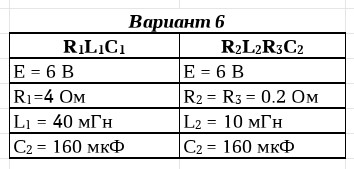
\includegraphics[width=1.2\textwidth]{table1.jpg}}

        Найдем частоту резонанса по току и напряжению:
        $$f_{PH} = \frac{1}{2\pi\sqrt{L_1C_1}} = 62 Hz $$ 
        $$f_{PT} = \frac{1}{2\pi\sqrt{L_2C_2}}\sqrt{\frac{\frac{L_2}{C_2} - R_2^2}{\frac{L_2}{C_2} - R_3^2}} = 125 Hz$$

        При резонансе по напряжению:
        $$I_o = \frac{U}{R+(2\pi f L - \frac{1}{2\pi f C})} \frac{U}{R} = 1.5 A$$
        $$ $$
        $$U_R = I_o R = 6\ V$$
        $$U_C = \frac{1}{2\pi f_{PH} C} = 16 \ V$$
        $$U_L =2\pi f_{PH} L = 15.6 \ V $$

        При резонансе по току:
        $$U_C = \frac{1}{2\pi f_{PH} C} = 16 \ V$$
        $$U_L =2\pi f_{PH} L = 15.6 \ V $$

        $$X_L = 7.9 \ \Omega$$
        $$X_C = 8 \ \Omega$$
        $$\varphi_1 = \arctan\frac{X_L}{R_2} = 88.55^\circ$$
        $$\varphi_2 = -\arctan\frac{X_C}{R_2} = -88.57^\circ$$

        $$Z_1 = R_2 + X_L = 8.1 \ \Omega$$
        $$Z_2 = R_2 + X_C = 8.2 \ \Omega$$

        $$I_1 = \frac{E}{Z_1} = 0.740 \ A$$
        $$I_2 = \frac{E}{Z_2} = 0.730 \ A$$
        $$I = \frac{E}{Z_1 + Z_2} = 0.368 \ A$$

    \section*{Задание 2. Построение векторных диаграмм}
        Векторная диаграмма для резонанса по напряжению:

        {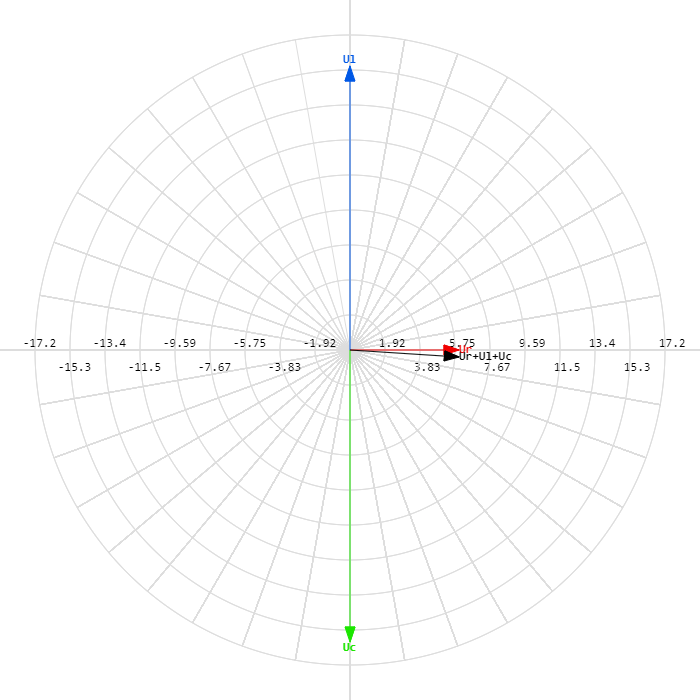
\includegraphics[width=0.8\textwidth]{vecPH.png}}

        Векторная диаграмма для резонанса по току:

        {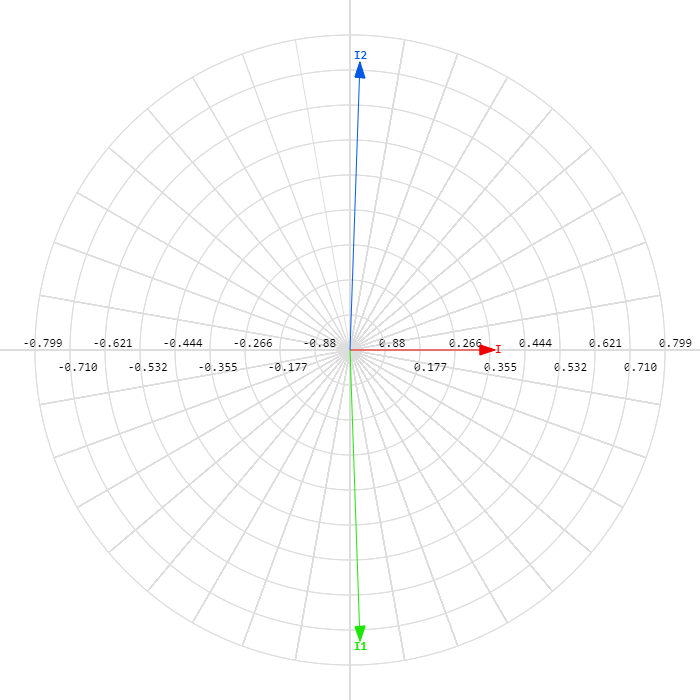
\includegraphics[width=0.8\textwidth]{vecPT.png}}


    \section*{Задание 3. Параметры колебательных контуров}
        Добротность:
        $$Q_{PH} = \frac{U_C}{U} = 2.7$$
        $$Q_{PT} = \frac{I_2\sin\varphi_2}{I} = 1.99$$

        Характеристическое сопротивление:
        $$\rho = \frac{U_c}{I_o} = 10.7 \Omega$$

        Характеристическая проводимость:
        $$\frac{1}{\rho} = \frac{I_2\sin\varphi_2}{U} = 0.07 \ \Omega^{-1}$$

        Полоса пропускания:
        $$\Delta f_{PH} \approx \frac{f_{PH}}{Q_{PH}} = 23 \ Hz$$
        $$\Delta f_{PT} \approx \frac{f_{PT}}{Q_{PT}} = 62.8 \ Hz$$ 


    \section*{Задание 4. Исследование резонансных явлений в колебательных контурах}
        {
            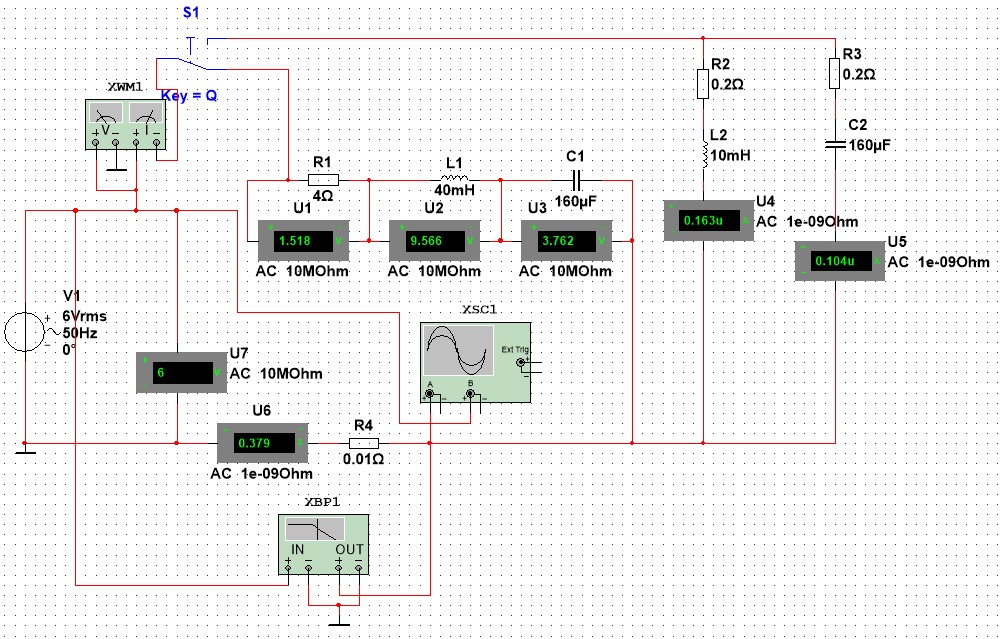
\includegraphics[width=0.8\textwidth]{Design.jpg}
        }
        
        {
            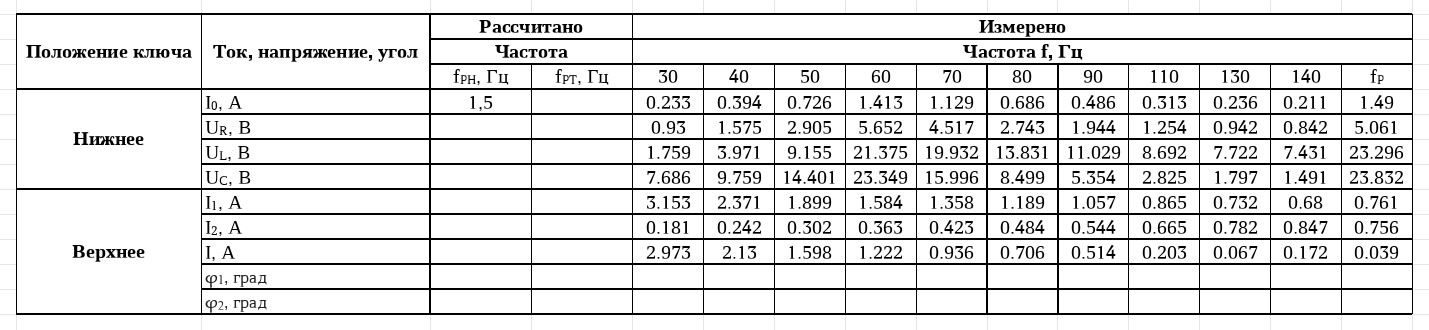
\includegraphics[width=0.8\textwidth]{table2.jpg}
        }


    \section*{Задание 5. Построение графиков}
        В последовательном соединении при наступлении определенной частоты возрастает напряжение на индуктивности и емкости.

        {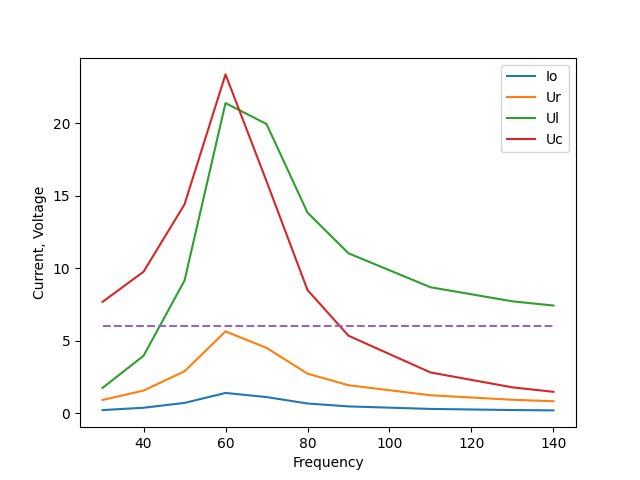
\includegraphics[width=0.8\textwidth]{graph1.png}}

        В параллельном соединении при наступлении определенной частоты токи в параллельных ветвях равны и в сумме превышают ток в цепи. 

        {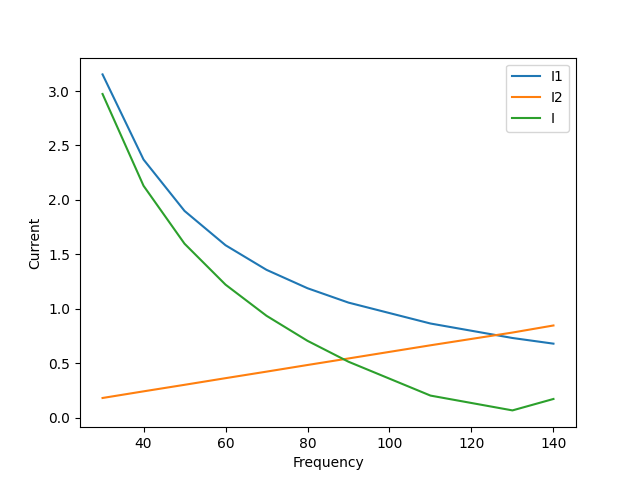
\includegraphics[width=0.8\textwidth]{graph2.png}}

        Векторная диаграмма при $f = 30 Hz$:

        {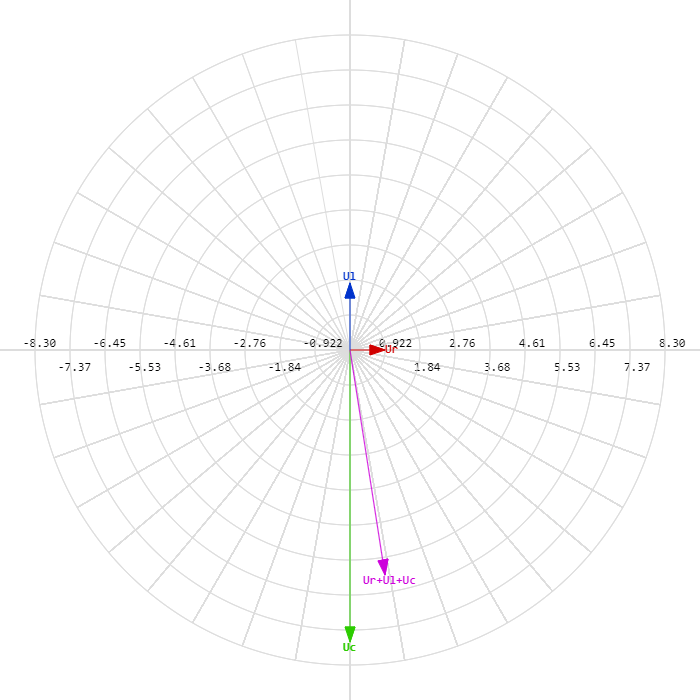
\includegraphics[width=0.8\textwidth]{vec30.png}}

        Векторная диаграмма при $f = 90 Hz$:

        {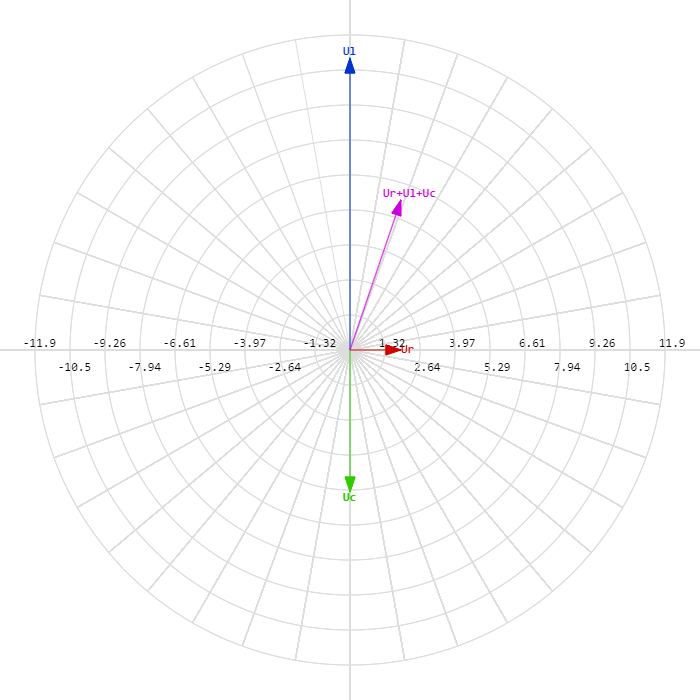
\includegraphics[width=0.8\textwidth]{vec90.png}}

    
    \section*{Вывод}
    В ходе данной лабораторной работы мы исследовали являения резонанса в последовательном и параллельном колебательных контурах
    и опрделили параметры колебательных контуров.




\end{document}